%%% Fiktivní kapitola s ukázkami tabulek, obrázků a kódu

\chapter{Zpracování dat}

Na datové platformě jsou real-time data o vozidlech dostupná do historie řádově jednotek minut, což je naprosto nedostatečné pro jakékoliv pozdější využití. Hlavně pro počítání statistik nad daty je potřeba zřídit lokální databázi, která bude držet historická data, tak jak proudila ze zdroje. Navíc data jsou poskytována ve formátu \gls{json}, který svou povahou není zrovna úsporný co se do velikosti souboru týče. Proto je vhodné zvolit ukládání dat v jiném formátu.

\section{Databáze}

Tato práce využívá relační databázi obsluhovanou dotazovacím jazykem \gls{sql}. Tato databáze se skládá z 5 tabulek. Jsou jimi:

\begin{itemize}
	\item \verb-trips- všechny objevené tripy

		\begin{itemize}
			\item \verb-id_trip- unikátní identifikátor používaný v databázi

			\item \verb-trip_source_id- identifikátor tripu převzatý ze zdroje dat

			\item \verb-id_headsign- identifikátor nápisu pro daný trip

			\item \verb-current_delay- aktuální zpoždění tripu

			\item \verb-shape_dist_traveled- aktuální vzdálenost ujetá od výchozí stanice

			\item \verb-last_updated- čas poslední aktualizace, převzatý ze zdroje dat

			\item \verb-trip_no- číslo dané linky
		\end{itemize}

	\item \verb-headsigns- nápisy nad vozidlem, cílová stanice

		\begin{itemize}
			\item \verb-id_headsign- unikátní identifikátor nápisu

			\item \verb-headsign- text nápisu
		\end{itemize}

	\item \verb-trip_coordinates- všechna historická real-time data

		\begin{itemize}
			\item \verb-id_trip- identifikátor tripu, ke kterému se záznam váže

			\item \verb-lat- zeměpisná šířka polohy vozidla

			\item \verb-lon- zeměpisná délka polohy vozidla

			\item \verb-inserted- čas vložení záznamu

			\item \verb-delay- zpoždění zachycené v poslední projeté stanici před pořízením záznamu

			\item \verb-shape_dist_traveled- vzdálenost ujetá od výchozí stanice tripu

		\end{itemize}

	\item \verb-stops- všechny zastávky

		\begin{itemize}
			\item \verb-id_stop- unikátní identifikátor zastávky

			\item \verb-trip_source_id- identifikátor zastávky převzatý ze zdroje dat

			\item \verb-parent_id_stop- identifikátor rodičovské zastávky, pokud existuje

			\item \verb-stop_name- název zastávky

			\item \verb-lat- zeměpisná šířka polohy zastávky

			\item \verb-lon- zeměpisná délka polohy zastávky

		\end{itemize}

	\item \verb-rides- trasa každého tripu, seznam zastávek s časy odjezdů a příjezd tvořící jízdní řád

	\begin{itemize}
		\item \verb-id_stop- identifikátor tripu

		\item \verb-id_stop- identifikátor zastávky

		\item \verb-arrival_time- čas příjezdu tripu do zastávky

		\item \verb-departure_time- časodjezduu tripu ze zastávky

		\item \verb-shape_dist_traveled- vzdálenost zastávky od výchozí zastávky tripu

	\end{itemize}

\end{itemize}

Atributy se jménem *source\_id jsou pravděpodobně unikátní identifikátor entity ve zdroji dat, nicméně z dokumentace zdroje to nevyplývá.Také je toto id textový řetězec a ačkoli je tvořen pouze číslicemi a podtržítky, není nikde zaručeno, že jej lze převést na číselný ko'd. Takže pro lepší výkon databáze je použito automaticky generované id typu \gls{int}.

\bigbreak

Každá tabulka ma několik indexů, které zlepšují výkon databáze při vkládání a hledání dat. Obvzláště pokud je atribut označen jako unikátní, kde se při každém vložení ověřuje unikátnost.

\begin{figure}[p]\centering
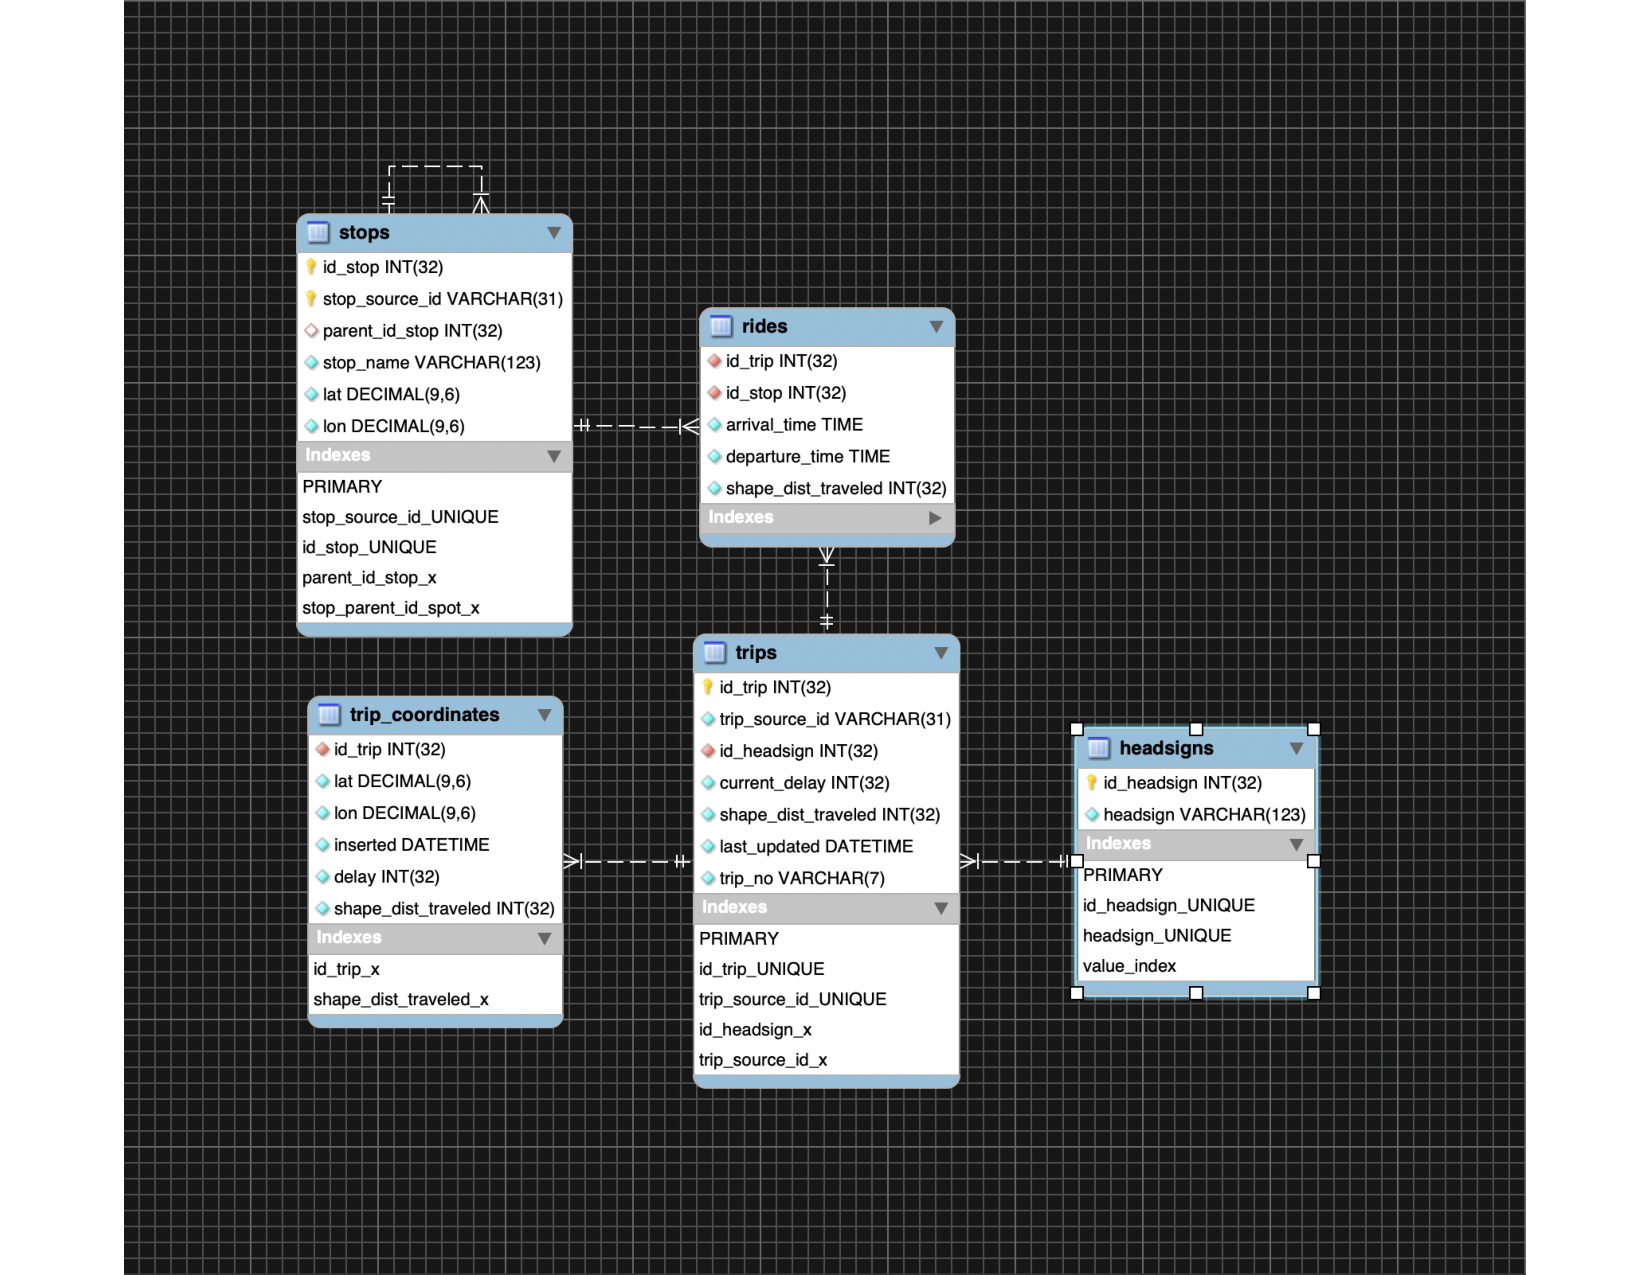
\includegraphics[width=140mm, height=140mm]{../img/eer_database}
% Příponu není potřeba explicitně uvádět, pdflatex automaticky hledá pdf.
% Rozměry také není nutné uvádět.
\caption{EER diagram databáze.}
\label{obr01:EER}

\end{figure}

TODO obrazek na bilem pozadi

Databáza je nastavená tak, aby umožnˇovala získat všechny potřebné informace o vozidlech, ale hlavně přístup k historickým real-time datům a to separovaně pro dvojci refenčních bodů.

TODO SQL dotazy na sestavení celé databaze jsou definovana v priloze, napsat to jako odstavec nebo jak se toto uvadi?

\subsection{Obsluha databáze}

Tato databáze je plněna skriptem jehož algoritmus postupně využívá všechna dostupná data z datové platformy následovně.

\bigbreak

Algoritmus:
\begin{code}[frame=none]
načti všechny dostupné zastávky
dokud skrip běží
	načti aktuální polohy vozidel
	pro každé nalezené vozidlo
		pokud trip vozidla je známí
			aktualizuj data
		jinak
			stáhni informace o tripu
			vlož trip
			zpracuj a vlož jízdu tripu
\end{code}

\bigbreak

Protože všechny infomace ukládané do databáze jsou důležité pro hlavní cíl této práce, tak pokud se vyskytne trip, který neobsahuje některou z požadovaných infomarcí je pak automaticky zahozen.

\bigbreak

Nejčastěji chybějící atribut je zpoždění v poslední zastávce, toto je nutné vědět pro počítání zpoždění mezi refenrečními body (zastávkami). Absence této informace může být způsobena tím, že vozidlo vůbec nevysílá data potřebnák k jejím dopočtení, pak nemá smysl jej do databáze zahrnovat. Nebo vozidlo už vysílá, ale ještě nezahájilo jízdu, tedy nemá žádnou poslední projetou zastávku, v takovém případe budou data ignorována až do doby příchodu první relevantní informace.

\bigbreak

Vkládání dat je řešeno pomocí databázových transakcí tak, aby stav databáze byl vždy konzistentní. Tedy pokud nejsou poskytnuta data ve formátu, který skript akceptuje, nebo nějaké povinné atributy chybí. Vložení celého tripu nebude provedono.

\bigbreak

Mimo popsanou databázi se do určeného adresáře ukládají trasy jednotlivých tripů. Tyto data jsou používány jen pro vykreslení na mapu, proto není nutné je držet v hlavní databázi.

\bigbreak

 Stejně tak i aktuální polohy vozidel jsou mimo databázi zapisovány do souboru, který je určen a formátován pro čtení webovou aplikací. Aktualizace tohoto souboru je provedena přednostně ihned po načtení real-timových dat.
